\documentclass[11pt]{article}

\usepackage[letterpaper,margin=1in]{geometry}
\usepackage{amsmath,amssymb}
\usepackage{booktabs}
\usepackage{graphicx}
\usepackage[hidelinks]{hyperref}
\usepackage[numbers,sort&compress]{natbib}
\usepackage{xcolor}
\usepackage{enumitem}
\usepackage{float}
\usepackage{microtype}
\usepackage{array}
\usepackage{algorithm}
\usepackage{algpseudocode}
\usepackage{caption}
\captionsetup{font=small,labelfont=bf,skip=3pt}
\newcolumntype{L}[1]{>{\raggedright\arraybackslash}p{#1}}
\setlength{\parskip}{2.5pt}
\setlength{\parindent}{0pt}
\setlist{nosep,leftmargin=1.4em}
\setlength{\textfloatsep}{6pt plus 2pt minus 2pt}
\setlength{\abovedisplayskip}{4pt plus 2pt minus 2pt}
\setlength{\belowdisplayskip}{4pt plus 2pt minus 2pt}
\setlength{\floatsep}{6pt plus 2pt minus 2pt}
\setlength{\intextsep}{6pt plus 2pt minus 2pt}
\newcommand{\confirm}[1]{\textbf{\textcolor{red}{[#1]}}}
\newcommand{\Ex}{\mathbb{E}}
\DeclareMathOperator*{\argmax}{arg\,max}

\title{Spectral Attribution Stability in Radar-Based Micro-Doppler Gesture Recognition Under Frequency-Domain Perturbation}

\author{
  Adedeji Oludayo \\
  Department of Computer Science, Bowie State University \\
  \texttt{oludayoa0130@students.bowiestate.edu}
}

\date{COSC 750 Pattern Recognition I --- Fall 2026 --- Stage 3 of 4: Methodology and Baselines}

\begin{document}
\maketitle
\vspace{-1.6em}

\begin{abstract}
Radar gesture recognizers are judged by accuracy, and their explanations are usually a single attribution map shown as a figure. This project asks whether those maps stay put when the radar signal changes in realistic ways. On the Google Soli data I train a CNN and an RBF-SVM under a user-grouped 4-fold protocol, explain both on a shared 8$\times$8 Doppler--time grid, apply band masking, magnitude smoothing and a noise-floor shift, and measure how far the maps move on sequences that every model still classifies correctly. A map change counts only if it exceeds the seed-to-seed floor. The literature review (Stage 2) found that realistic corruption has been studied through accuracy and explanation fragility only under adversarial attack. This stage adds the formal problem, the measurement protocol, five baselines and first stability results. Mean accuracy over 4 folds $\times$ 5 repeats is 9.1\% (majority), 64.1\% (PCA + Gaussian Bayes), 81.2\% (RBF-SVM), 89.4\% (project CNN) and 91.2\% (CNN--RNN); a random split would have lifted the SVM to 93.8\%. The hypothesis that CNN maps leave their floor before accuracy falls is not supported: it held in 0 of 1{,}200 run-level cases, and Grad-CAM maps cross the floor only after accuracy has fallen by about 9 points or more. The SVM's maps are steadier, but its accuracy is far more sensitive to a noise-floor shift. CNN and SVM maps do not agree with each other (Spearman $-0.15$).
\end{abstract}

\noindent\textbf{Keywords:} pattern recognition; micro-Doppler radar; gesture recognition; attribution; explanation stability; support vector machine

%==================================================================
\section{Introduction}
A micro-Doppler gesture recognizer maps an input $x$ built from range-Doppler maps to one of $c$ gesture classes $\omega_1,\dots,\omega_c$. Accuracy on Soli is already high, so the harder question is whether a correct prediction is correct for reasons that survive ordinary changes in the signal chain. Noise floor, spectral leakage and windowing all reshape a micro-Doppler map. If an explanation moves under mild filtering while the label stays put, anyone who tuned a gesture interface by reading that explanation tuned it to something unstable.

\textbf{Data, as corrected in this stage.} I use the \texttt{deep-soli} release of Soli~\citep{wang2016soli}: 5{,}500 HDF5 sequences of four-channel $32\times32$ range-Doppler frames in 12 classes. Eleven are gestures with 475 sequences each; the twelfth is a background class (275 sequences) that belongs to no user, so I leave it out ($n=5{,}225$ remain). A scan of all 5{,}500 files shows 28 to 145 frames per sequence (median 56), not the fixed 68 I stated in Stages 1 and 2, so every sequence is resampled to 32 frames. It also found no label that changes within a file, none that disagrees with its file name and no non-finite value, which closes the Stage 2 label check.

\textbf{Research question (unchanged from Stage 2).} \emph{On correctly classified Soli sequences, under three sensor-motivated frequency-domain perturbations at matched severity, how much do attribution maps of a CNN and an SVM change, and do they change measurably before accuracy falls?} \textbf{Hypothesis H:} for some perturbation and severity, the clean-versus-perturbed map similarity falls below the seed-to-seed floor while accuracy has dropped by less than 2 percentage points. This is my definition of a \emph{useful outcome}: a statistically significant map change does not count unless it also clears the floor and comes early, before accuracy gives the problem away.

\textbf{Course topics and contributions.} Bayes decision theory and 0--1 risk, Gaussian density estimation with PCA (B1a), a kernel SVM (B1b), convolutional and recurrent networks (CNN, B2) and the bias--variance argument behind the seed floor. Contributions: (1)~a protocol for attribution stability on radar spectra that conditions on correct predictions, reports retention, and compares every change with a floor; (2)~five baselines on a user-grouped split, with variance and a measured leakage gap of 12.6 accuracy points; (3)~first stability results, one of them negative, and a repository that rebuilds the baseline table with one command.

%==================================================================
\section{Related Work}
\subsection{Search strategy}
\noindent I ran Boolean queries in IEEE Xplore (title and abstract), the ACM Digital Library (guest access) and Google Scholar, combining radar (\emph{radar, mmWave, micro-Doppler}), explanation (\emph{explainable, XAI, Grad-CAM, saliency, attribution}) and stability (\emph{robust*, stability, perturbation}) terms; assisted web search covered stability work outside radar (arXiv and Scopus were not searched). I kept 2001--2026 peer-reviewed papers and identifiable preprints on radar gesture or activity recognition, attribution methods, or measured explanation stability or corruption robustness, and dropped records with unconfirmable authors, venue or DOI and papers where ``saliency'' means something else (SAR, beamforming, 6G). IEEE returned 89 records (87 papers), ACM 14, Scholar about 16{,}200 and 584 for two variants; $N_1=111$ records were screened (IEEE 87, ACM 14, Scholar 10) and $N_3=24$ are cited.

\subsection{Taxonomy and the three threads}
Fig.~\ref{fig:tax} sorts the sources into three threads that rarely meet.
\textbf{Radar recognition.} Classical work pairs hand-built micro-Doppler features with an SVM~\citep{kim2009activity}; deep models followed: a CNN on micro-Doppler images~\citep{kim2016handgesture}, a CNN--RNN on Soli sequences~\citep{wang2016soli}, ResNet-18 with an LSTM~\citep{zhang2022resnetlstm}, and recent work on objects, activity and cheap reservoirs~\citep{attygalle2021nointerface,tan2024har,sano2026esn}. Orthogonal-moment features are reported as more noise-robust than CNNs on a public activity set~\citep{vannifterik2024moments}.
\textbf{Attribution methods.} Grad-CAM~\citep{selvaraju2017gradcam} and Integrated Gradients~\citep{sundararajan2017ig} explain neural models; permutation importance~\citep{fisher2019allmodels} covers models without gradients.
\textbf{Stability of explanations.} Some saliency maps barely depend on the model~\citep{adebayo2018sanity}; small label-preserving changes can move an interpretation~\citep{ghorbani2019fragile}; robustness, infidelity and relative-stability measures exist~\citep{alvarezmelis2018robustness,yeh2019infidelity,agarwal2022rethinking}, with one training-time fix~\citep{chen2019robustattr} and a consistency check on time series~\citep{balestra2023saliency}. SSIM~\citep{wang2004ssim} compares two maps.
\textbf{Where the threads touch radar.} Non-adversarial corruption of micro-Doppler spectra has been measured, but through accuracy, with saliency shown only as figures~\citep{zhou2024corruption}. Explanations on radar have been tested under adversarial attack~\citep{ozbulak2021radaradversarial,chen2024sar}, and attributions on radar activity data used for privacy, not stability~\citep{zakariyya2025idg}.

\begin{figure}[!tb]
\centering
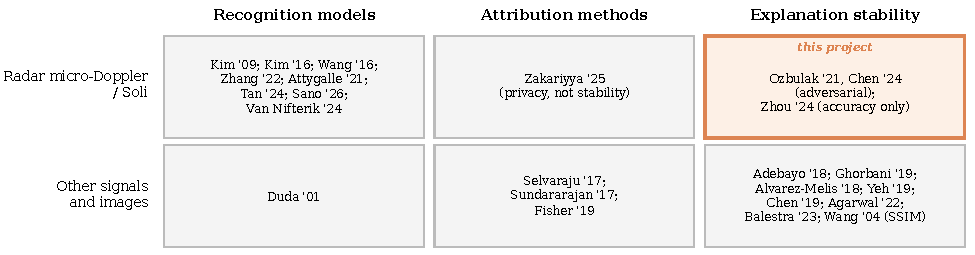
\includegraphics[width=0.96\textwidth]{figures/taxonomy.pdf}
\caption{Taxonomy of the 24 cited works by data domain (rows) and topic (columns). The orange cell, explanation stability on radar spectra under non-adversarial change, is where this project sits.}
\label{fig:tax}
\end{figure}

\begin{table}[!tb]
\centering
\footnotesize
\setlength{\tabcolsep}{3pt}
\begin{tabular}{@{}L{2.9cm}L{4.0cm}L{3.2cm}L{5.0cm}@{}}
\toprule
\textbf{Work} & \textbf{Method} & \textbf{Data} & \textbf{Limitation for our question} \\
\midrule
Wang '16 \citep{wang2016soli} & CNN--RNN, end to end & Soli (introduces it) & Accuracy only; no explanation study \\
Sano \& Tanaka '26 \citep{sano2026esn} & Echo state network + SVM/ridge & Soli (11 classes), Dop-NET & 98.84\% random split vs.\ 92.62\% leave-one-subject-out \\
Zhou '24 \citep{zhou2024corruption} & Nine non-adversarial corruptions; ResNet-18 and others & Glasgow indoor, ZJU aquatic (FMCW) & Accuracy-based; saliency qualitative only \\
Ozbulak '21 \citep{ozbulak2021radaradversarial} & Grad-CAM + adversarial attacks & Radar activity recognition & Adversarial only; not Soli gestures \\
Van Nifterik '24 \citep{vannifterik2024moments} & Orthogonal moments vs.\ CNN & Public radar HAR set & Noise robustness; no attribution stability \\
\bottomrule
\end{tabular}
\caption{Key works compared. Accuracy figures appear only where I read them in the source; the rest are placed in Fig.~\ref{fig:tax}.}
\label{tab:cmp}
\end{table}

\subsection{Critical synthesis, gap and positioning}
Radar models are shown robust by accuracy and explanations fragile by attack, but the two kinds of evidence never meet, so nobody knows whether a model that survives realistic corruption still decides for the same reasons. Deep models beat hand-built features on radar gestures, and explanation methods exist for gradient and non-gradient models. Whether attribution maps deserve trust at all is contested~\citep{adebayo2018sanity,ghorbani2019fragile,yeh2019infidelity}, on image evidence that is rarely checked on spectra, where neighbouring bins are strongly correlated. Three weaknesses recur: Soli results are not comparable across papers (\citet{sano2026esn} report a 6-point drop from random to leave-one-subject-out splits; \citet{zhang2022resnetlstm} state their headline accuracy on the training set); radar explanation tests use attacks, a worst case, or realistic corruption with accuracy only~\citep{zhou2024corruption}; and few studies give an explanation-variance floor, so a change cannot be told from retraining noise.

\textbf{Gap.} No study quantifies how attribution maps of a Soli-style classifier move under non-adversarial, sensor-motivated frequency-domain changes, restricted to correct predictions and under a user-grouped split. I take the stability idea from \citet{agarwal2022rethinking} and \citet{yeh2019infidelity}, the maps from \citet{selvaraju2017gradcam}, \citet{sundararajan2017ig} and \citet{fisher2019allmodels}, and the case for realistic corruptions from \citet{zhou2024corruption}, whose Doppler, STFT and noise corruptions my perturbations echo. The contribution is the measurement, not a new attribution method.

%==================================================================
\section{Problem Formulation}\label{sec:form}
\textbf{Inputs and labels.} Each sequence is reduced to a Doppler--time map $x\in\mathbb{R}^{T\times D}$, $T=D=32$ ($d=1024$): the mean over the four receive channels and over the range axis of each $32\times32$ frame, after linear resampling to $T$ frames. Resampling is needed because sequences run from 28 to 145 frames while the CNN, SVM features, 8$\times$8 explanation grid and perturbation bins all assume one fixed shape; padding or cropping would add fake zeros or cut gestures, and a variable-length model would give B2 a different input from the other methods. Doppler is the column axis; on the data the column profile has a sharp central peak at bin 16 and the row profile does not. There are $c=11$ classes with equal priors $P(\omega_i)=1/11$, and $\mathcal D=\{(x_k,y_k,u_k)\}_{k=1}^{n}$, $n=5{,}225$, where $u_k$ is the user (ten users) who produced sequence $k$.

\textbf{Decision rule.} With 0--1 loss $\lambda(\alpha_i\mid\omega_j)=\mathbf 1[i\neq j]$ the risk of action $\alpha_i$ is $R(\alpha_i\mid x)=1-P(\omega_i\mid x)$, so the Bayes rule is
\begin{equation}
\hat\omega(x)=\argmax_{i} P(\omega_i\mid x)=\argmax_i g_i(x).
\label{eq:bayes}
\end{equation}
Each model learns its own $g_i$: Gaussian class-conditionals on PCA scores (B1a), the one-vs-rest scores of an RBF-SVM (B1b), or network logits (CNN, CNN--RNN). Accuracy estimates $1-R$; the classes are nearly balanced, so macro-F1 is a check, not a different target. Sequences from one user are correlated, so independence holds across users, not sequences, and the target is the expected risk on \emph{unseen users}.

\textbf{Attributions and perturbations.} For a trained model $f$, input $x$ and class $y$, an attribution map $a_f(x,y)\in\mathbb{R}^{G\times G}$ lives on an $8\times8$ grid of time blocks and Doppler bands ($G=8$; each cell is 4 frames by 4 Doppler bins), the same grid for every model. A perturbation $\pi_{\kappa,s}$ has a kind $\kappa\in\{\text{band mask},\text{smooth},\text{floor shift}\}$ and a strength $s\in[0,1]$.

\textbf{Quantities.} Let $\mathcal C$ be a cohort of test sequences that all models classify correctly, $\tilde a$ a normalised map (Eq.~\ref{eq:norm}) and $\rho$ a similarity. Stability and the floor are
\begin{equation}
\Delta_{\kappa}(s)=\Ex_{x\in\mathcal C}\,\rho\big(\tilde a_f(x,y),\,\tilde a_f(\pi_{\kappa,s}x,y)\big),
\qquad
F=\Ex_{x\in\mathcal C}\,\rho\big(\tilde a_{f_A}(x,y),\,\tilde a_{f_B}(x,y)\big),
\label{eq:stab}
\end{equation}
where $f_A,f_B$ differ only in their training seed and $F$ is evaluated on clean input. With $A_\kappa(s)$ the drop in test accuracy, H says: for some $\kappa,s$, $\Delta_\kappa(s)<F$ and $A_\kappa(s)<2$ points.

\textbf{Assumptions.} Independence across users; the pooled Doppler--time map as an adequate stand-in for the signal chain (untested, see Section~\ref{sec:res}); an $8\times8$ grid fine enough to localise evidence. I test the labels, the Doppler axis, split leakage, and (by sanity checks) that maps depend on what the model learned.

%==================================================================
\section{Method}\label{sec:method}
\begin{figure}[!tb]
\centering
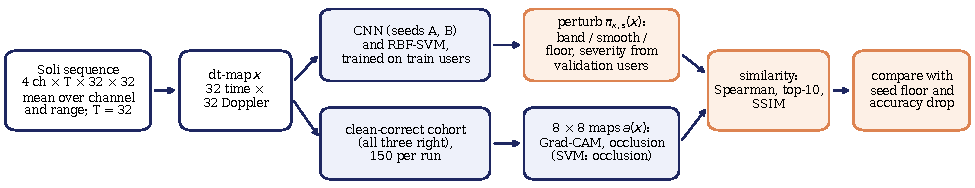
\includegraphics[width=\textwidth]{figures/pipeline.pdf}
\caption{Pipeline from a Soli sequence to a stability verdict. Blue: trained models and maps; orange: perturbation and comparison with the floor. Severities are fitted on validation users only.}
\label{fig:pipe}
\end{figure}

\textbf{Models.} Two CNNs with different seeds ($f_A,f_B$) and one SVM ($h$) are trained on the training users of a fold. The CNN has three conv--BatchNorm--ReLU blocks and two max-pools, so its last map is $8\times8$ like the grid, then global average pooling and a linear layer. The SVM sees the mean and standard deviation of every grid cell (128 features), standardised.

\textbf{Maps.} Grad-CAM at the last conv layer for the true-class logit (already $8\times8$), and occlusion for both models: one grid cell is replaced by the training mean intensity and the drop in the true-class score is recorded. I use occlusion for the SVM instead of the Stage 2 permutation importance, which is dataset-level; occlusion is local, so both models share one definition on the same cells. Maps are normalised per sequence,
\begin{equation}
\tilde a=\max(a,0)\Big/\textstyle\sum_{ij}\max(a_{ij},0)\quad(\text{uniform if the sum is }0),
\label{eq:norm}
\end{equation}
so only the distribution of positive evidence matters.

\textbf{Perturbations} act along the Doppler axis of $x$. \emph{Band mask} multiplies a centred band of $2+\mathrm{round}(14s)$ bins by $1-s$; \emph{smooth} applies a Gaussian filter of width $6s$ bins (coarser Doppler resolution); \emph{floor shift} clips values below $0.5\,s$ times the sequence peak (a raised noise floor). Strengths are not comparable across kinds, so each kind is calibrated by bisection on validation users in two ways: to a target mean input SSIM $\tau\in\{0.99,0.97,0.95,0.85,0.75,0.65\}$, and to a target drop $\delta\in\{1,2,5,10\}$ points in the CNN's validation accuracy.

\textbf{Similarity.} Spearman rank correlation over the 64 cells ($\rho$, the primary measure; scale-free and not dominated by a few cells), top-10 cell overlap, and SSIM with a $3\times3$ window. The three order the conditions alike (rank correlation 0.89 and 0.88 with $\rho$ over the 90 summary rows), so I report $\rho$.

\begin{algorithm}[!tb]
\caption{Attribution stability for one fold and repeat}\label{alg:stab}
\begin{algorithmic}[1]
\State Fit $f_A,f_B$ (seeds $\sigma,\sigma{+}1000$) and $h$ on train users; choose hyper-parameters on validation users
\State $\mathcal C\leftarrow$ 150 random test sequences that $f_A,f_B,h$ all classify correctly
\State Clean maps $\tilde a_{f_A},\tilde a_{f_B},\tilde a_h$ on $\mathcal C$; floors $F$; sanity maps (random-weight CNN, label-permuted SVM)
\For{each $\kappa$ and target level ($\tau$ or $\delta$)}
  \State Pick $s$ by bisection on validation users; perturb $\mathcal C$ and all test users; record test accuracy of $f_A$ and $h$
  \State Recompute maps; $\rho$, top-10, SSIM against the clean maps, over all of $\mathcal C$ and over the retained sequences
\EndFor
\end{algorithmic}
\end{algorithm}

\textbf{Why it should work.} \emph{Conditioning:} Eq.~\eqref{eq:bayes} makes the decision depend on $\argmax_i g_i$, so if the label flips any map of the true class changes for a trivial reason. A clean-correct cohort removes that cause, and the retention $r_\kappa(s)=|\{x\in\mathcal C:\hat\omega(\pi_{\kappa,s}x)=y\}|/|\mathcal C|$ shows how selective the survivors are. \emph{Floor:} a map is an estimator that depends on a finite training sample and on initialisation, so it has variance; $F$ measures it, and a change smaller than $1-F$ cannot be told from retraining noise. \emph{Severity matching:} SSIM makes kinds comparable in how much structure they destroy, the accuracy target in how much decision-relevant evidence; I added the second when the first did not track accuracy. \emph{SVM:} for an RBF kernel each binary decision function $\sum_i\alpha_i y_i k(x_i,\cdot)+b$ is Lipschitz in feature space with constant at most $(\sum_i|\alpha_i|)\sqrt{2\gamma}$, since $\|\phi(x)-\phi(x')\|^2=2-2k(x,x')\le2\gamma\|x-x'\|^2$, so small input changes move its scores by a bounded amount. The bound is loose, and scikit-learn's one-vs-rest score adds integer vote counts that can jump, so it gives direction only. For a ReLU network no useful bound exists, and Grad-CAM gradients change across activation boundaries, the fragility \citet{ghorbani2019fragile} describe.

\textbf{Complexity.} Training: Bayes $O(nd^2+nd'^2+c\,d'^3)$ ($d=128$ features, $d'$ PCA components); SVM between $O(n^2d)$ and $O(n^3)$; CNNs $O(E\,n\,\mathrm{FLOPs})$ for $E\le30$ epochs. Grad-CAM costs one forward and one backward pass, occlusion $G^2=64$ extra forward passes per sequence; one stability run took 41--58 s.

%==================================================================
\section{Experimental Setup}\label{sec:setup}
\textbf{Data and splits.} The \texttt{deep-soli} code is MIT-licensed and the dataset license is not stated separately (cited via~\citet{wang2016soli}). The README's session arrangement gives ten users: A has six sessions (0, 1, 4, 7, 13, 14; 2{,}750 sequences, 53\% of the data) and nine users have one session of 275 sequences (session 13 is in both README lists, so A is also the tenth cross-user subject). All sessions of a user stay together. The folds are $\{$A$\}$, $\{$u2,u3,u5$\}$, $\{$u6,u8,u9$\}$, $\{$u10,u11,u12$\}$, with 2{,}750, 825, 825 and 825 test sequences. In each of 5 repeats per fold, 2 validation users are drawn from the rest of the pool (never A) and the others train (1{,}925 sequences in fold 0, 3{,}850 otherwise). Code asserts that no user or session appears in two of train, validation and test; normalisers are fitted on training data only. A random stratified split (3{,}657/784/784) gives a deliberately leaky SVM reference.

\textbf{Baselines.} \emph{B3 majority class:} the floor. \emph{B1a PCA + Gaussian Bayes:} the course's optimal-under-assumptions reference~\citep{duda2001pattern}, my own code with class covariances shrunk toward the pooled one so they stay invertible (tuned: PCA dimension, shrinkage). \emph{B1b RBF-SVM} (scikit-learn) on the 128 block features, in the line of~\citet{kim2009activity} (tuned: $C,\gamma$). \emph{B2 CNN--RNN:} a per-frame CNN on the four-channel range-Doppler frames followed by a GRU, after~\citet{wang2016soli}; it is my re-implementation, not their code or exact architecture, so it reproduces a published \emph{design}, not their numbers (tuned: hidden size, learning rate). It reads the full range-Doppler sequence; all other methods read the Doppler--time map. \emph{Project CNN:} the model of Section~\ref{sec:method} (tuned: width, learning rate, weight decay). Every method gets the same splits and the same budget of 4 configurations, chosen by validation-user accuracy; CNNs train for at most 30 epochs (Adam, batch 64, early stopping with patience 6). The optional ResNet-18 + LSTM baseline of Stage 2 was dropped for lack of time.

\textbf{Protocol and metrics.} Each fold is repeated 5 times with different validation users and seeds (seed $=100\cdot\text{fold}+\text{repeat}$; the second CNN uses $+1000$). I report accuracy and macro-F1 as mean $\pm$ sd over the 5 repeats of the fold-averaged score, plus per-fold means and the sd across folds, the honest measure of movement between users. Significance uses paired $t$-tests on the four fold means ($n=4$; runs within a fold share test users and are not independent); with four comparisons I read $p<0.0125$ as significant. Runs used Google Colab with one CUDA GPU and Python 3.13; a tuned fit took about 1 s (Bayes, SVM), 2--17 s (CNN) and 72--144 s (CNN--RNN), and all baselines took 39 min.

\emph{Fixed before any test-user result was seen:} split design, baselines, grids and budget, accuracy and macro-F1, the three similarity measures, the floor, and the 2-point criterion in H. \emph{Changed after a first stability run, hence exploratory:} two defective perturbations were redefined (the first noise-floor shift changed nothing; band masking collapsed three severity levels into one); milder SSIM levels and the accuracy-matched calibration were added; the SVM got its own floor (a refit on a random 80\% of its training sequences) instead of the CNN's; and tests moved from 20 runs to four folds. None of this touched hyper-parameter selection or the baseline table.

\textbf{Implementation and reproducibility.}\label{sec:repro} Code: \confirm{GitHub URL} (Python; PyTorch, scikit-learn, scikit-image; \texttt{requirements.txt} and \texttt{environment.yml}). \texttt{make reproduce DATA=SoliData.zip DEVICE=cuda} builds the cache, runs every baseline and writes the table (the Colab run called the same scripts one by one); \texttt{make stability} runs the attribution experiment; \texttt{make smoke} checks the whole pipeline on synthetic data in under a minute; 14 unit tests cover splits, perturbations, metrics and occlusion. The code was written with Claude (see the disclosure), none is taken from the \texttt{deep-soli} repository, and library versions are those pip resolved on Colab (not pinned). GPU kernels are not deterministic, so reruns differ slightly: a first complete run gave 89.0 (CNN) and 90.7 (CNN--RNN) against 89.4 and 91.2 reported here; Bayes, SVM and majority were identical.

%==================================================================
\section{Results}\label{sec:res}
\subsection{Baselines}
Both neural models beat the SVM in every fold (+8.2 and +10.0 points, $p=0.005$ each) and the Bayes classifier trails it by 17 points ($p=0.009$); all three survive the four-test correction. The CNN--RNN leads the project CNN by 1.8 points in only 2 of 4 folds ($p=0.38$), so the two cannot be separated. The $\pm$ over repeats (0.5--1.8) understates the real uncertainty: results vary by 2.2--5.5 points (sd) between folds, and fold 0 (user A, smallest training set) is the CNN's worst (85.9). Validation users are easier than test users (CNN 93.1 vs.\ 89.4). Leakage is large: the SVM scores 93.8 on a random split and 81.2 on unseen users, a 12.6-point gap a random split would have passed off as skill. In repeat 0 the CNN's recall is above 0.9 for eight of eleven classes; its main errors send class 0 (38\%) and class 3 (30\%) to class 10.

\begin{table}[!tb]
\centering
\small
\setlength{\tabcolsep}{3.6pt}
\begin{tabular}{@{}lccccccccc@{}}
\toprule
 & \multicolumn{2}{c}{Accuracy (\%)} & Macro-F1 & \multicolumn{4}{c}{Accuracy by fold} & \multicolumn{2}{c}{vs.\ SVM} \\
\cmidrule(lr){2-3}\cmidrule(lr){5-8}\cmidrule(l){9-10}
Method & mean $\pm$ sd$_{\rm rep}$ & sd$_{\rm fold}$ & (\%) & F0 & F1 & F2 & F3 & $\Delta$ pts & $p$ \\
\midrule
B3 majority class & 9.1 $\pm$ 0.0 & 0.0 & 1.5 $\pm$ 0.0 & 9.1 & 9.1 & 9.1 & 9.1 & $-$72.1 & --- \\
B1a PCA + Gauss.\ Bayes & 64.1 $\pm$ 1.8 & 5.5 & 63.5 $\pm$ 1.9 & 70.0 & 56.7 & 65.7 & 63.9 & $-$17.1 & 0.009 \\
B1b RBF-SVM & 81.2 $\pm$ 1.0 & 2.5 & 80.9 $\pm$ 1.0 & 79.5 & 78.9 & 82.0 & 84.4 & --- & --- \\
Project CNN & 89.4 $\pm$ 0.5 & 2.4 & 89.0 $\pm$ 0.6 & 85.9 & 90.1 & 90.6 & 91.0 & +8.2 & 0.005 \\
B2 CNN--RNN & \textbf{91.2 $\pm$ 1.2} & 2.2 & \textbf{91.2 $\pm$ 1.2} & 92.2 & 88.3 & 93.6 & 90.8 & +10.0 & 0.005 \\
\midrule
SVM, random split (leaky) & 93.8 $\pm$ 1.2 & --- & --- & \multicolumn{4}{c}{(5 random splits)} & +12.6 & --- \\
\bottomrule
\end{tabular}
\caption{Test accuracy on held-out users, 4 folds $\times$ 5 repeats. sd$_{\rm rep}$: sd over the 5 repeats of the fold-averaged accuracy; sd$_{\rm fold}$: sd across the four folds. $p$: paired $t$-test on fold means against the SVM ($n=4$). F0 has one test user (2{,}750 sequences); F1--F3 have three users and 825 sequences each.}
\label{tab:main}
\end{table}

\subsection{Preliminary attribution-stability results}
\textbf{Sanity checks pass.} Against the trained maps, a random-weight CNN gives Spearman $-0.05\pm0.06$ (Grad-CAM) and $0.09\pm0.06$ (occlusion), and a label-permuted SVM $0.13\pm0.05$, all far below the floors, so the maps depend on what was learned. \textbf{Floors.} Two CNN seeds agree at $\rho=0.866\pm0.019$ (Grad-CAM) and $0.594\pm0.059$ (occlusion); two SVMs fitted on different 80\% subsets at $0.982\pm0.004$. Grad-CAM and occlusion on one CNN agree at 0.46, and CNN and SVM occlusion maps at $-0.15$ with a top-10 overlap of 0.011 against about 0.16 by chance, so maps of different models cannot be compared cell by cell and I compare stability \emph{within} each model.

\begin{figure}[!tb]
\centering
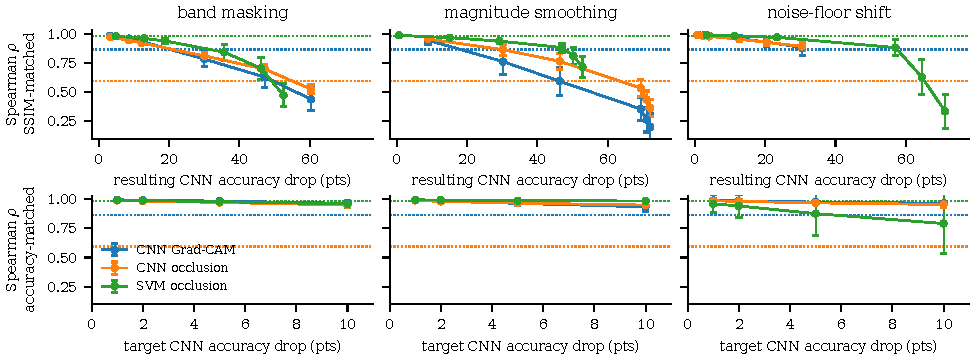
\includegraphics[width=\textwidth]{figures/stability.pdf}
\caption{Spearman similarity between clean and perturbed maps (mean $\pm$ sd over 20 runs). Top: severities matched by input SSIM, plotted against the resulting CNN accuracy drop. Bottom: severities calibrated to a CNN accuracy drop of 1, 2, 5 and 10 points. Dotted lines are the seed floors of the same colour.}
\label{fig:stab}
\end{figure}

\textbf{H is not supported for the CNN.} Over all conditions and runs (600 Grad-CAM and 600 occlusion cases) the CNN's map similarity was below its floor with an accuracy drop under 2 points in \emph{none}. For the SVM it happened in 11 of 600 cases, but its floor (0.982) leaves almost no room: a map change of 0.02 already counts. When CNN maps do leave their floor, accuracy is already gone (Table~\ref{tab:cross}): Grad-CAM crosses after the CNN has lost 9 to 30 points under smoothing and 12 to 30 under band masking, and not within the tested range under a noise-floor shift; occlusion maps cross only after 46 to 69 points. At the strength calibrated to a 10-point drop, CNN map similarity stays between 0.93 and 0.96 (Fig.~\ref{fig:stab}, bottom).

\begin{table}[!tb]
\centering
\footnotesize
\setlength{\tabcolsep}{2.5pt}
\begin{tabular}{@{}lccccccc@{}}
\toprule
 & \multicolumn{2}{c}{CNN drop (pts) where $\rho$ crosses floor} & \multicolumn{5}{c}{Strength calibrated to a 10-point CNN drop on validation users} \\
\cmidrule(lr){2-3}\cmidrule(l){4-8}
Perturbation & Grad-CAM (0.87) & occlusion (0.59) & CNN drop & CNN $\rho$ (GC / occ.) & SVM drop & SVM $\rho$ & SVM kept \\
\midrule
Band mask & 12--30 & 47--60 & 7.0 & 0.96 / 0.95 & 11.3 & 0.96 & 84\% \\
Smoothing & 9--30 & 46--69 & 10.2 & 0.93 / 0.95 & 2.1 & 0.98 & 94\% \\
Floor shift & not crossed ($\le$30) & not crossed ($\le$30) & 9.3 & 0.96 / 0.95 & 50.5 & 0.79 & 40\% \\
\bottomrule
\end{tabular}
\caption{Where maps leave the floor, and the SVM at the same strength. Crossing ranges run from the last SSIM level above the floor to the first below it (CNN accuracy drop at each); floors in brackets. Drops are on test users; kept: share of the 150-sequence cohort the SVM still gets right.}
\label{tab:cross}
\end{table}

\textbf{The models fail differently.} At strengths that cost the CNN about 10 points, smoothing barely touches the SVM (2.1 points), plausibly because its features pool several Doppler bins; band masking hurts both alike; the noise-floor shift is brutal for the SVM (50.5 points, 40\% of the cohort kept, $\rho=0.79\pm0.26$) and costs the CNN 9.3. \textbf{Selection effect.} Conditioning on survivors flatters stability: under smoothing at SSIM 0.65, Grad-CAM similarity is 0.20 over the cohort but 0.83 over the 17\% still correct, so failing sequences have maps that changed almost completely (about 0.07).

\textbf{Limits.} The perturbations act on the pooled Doppler--time map, not the raw signal chain, and are simulated. Linear resampling to 32 frames discards gesture duration and slightly smooths fast Doppler changes. The SVM score includes vote counts, which may explain its high floor. Twenty runs from four folds on one dataset is a small sample, and the accuracy-matched results are exploratory. \textbf{RQ3.} Over the 600 perturbed conditions per method, map similarity and CNN accuracy drop are rank-correlated at Spearman $-0.92$ (Grad-CAM), $-0.90$ (CNN occlusion) and $-0.93$ (SVM occlusion), and $-0.95$ to $-0.96$ on fold means. Both move with severity, so maps degrade \emph{with} accuracy; this does not show that they warn of it earlier. \textbf{Stage 4.} Physically grounded impairments (noise at a set SNR, low-Doppler clutter, channel gain mismatch) and natural shift across users; Integrated Gradients and a margin-based SVM score; a faithfulness check against the Doppler bins carrying gesture energy; equal SVM tuning effort; a protocol frozen before running.

%==================================================================
\section*{Response to Feedback}
\small
\textbf{Split and leakage (Stage 1).} User-grouped folds from the README's session arrangement, with asserts that no user or session crosses train, validation and test (Sec.~5); the leakage cost is measured (12.6 points). \textbf{Sample-level CNN maps versus dataset-level SVM importance (Stage 1); local SVM explanation (Stage 2).} Both models are explained locally by occlusion on the same $8\times8$ Doppler--time cells, with Grad-CAM as a second CNN map (Sec.~4). \textbf{Selection effect (Stage 1); retention (Stage 2).} One cohort is shared by both CNN seeds and the SVM, and retention and survivor-only similarity are reported (Sec.~6.2). \textbf{Useful outcome (Stage 1).} H needs a drop below a measured seed floor with under 2 points of accuracy loss. \textbf{Session identifiers (Stage 2).} The README gives sessions per user and they drive the split (Sec.~5). \textbf{Units, severity, normalisation, sanity checks, cross-model comparison (Stage 2).} Units are Doppler bins; severity is matched by SSIM and by accuracy drop; maps are sum-to-one normalised; sanity checks pass; cross-model agreement is near zero, so stability is compared within each model.

\textbf{Corrections to Stage 2.} Frames per sequence are 28--145, not 68; the background class is excluded; the random-plus-held-out-session plan became user-grouped folds (random split only as a leaky reference); B2 is the CNN--RNN, the CNN is the project model, ResNet-18 + LSTM was dropped; the SVM is explained by occlusion, not permutation importance; Spearman is the primary similarity.

%==================================================================
\section*{AI-Use Disclosure (Stage 3)}
\begin{table}[H]
\centering
\footnotesize
\begin{tabular}{@{}p{1.3cm}p{4.2cm}p{9.8cm}@{}}
\toprule
\textbf{Tool} & \textbf{Used for} & \textbf{Extent and verification} \\
\midrule
Claude & Repository code and tests, figures, drafting and revision of this paper's text & I ran every experiment on Colab and returned the outputs; every number here comes from those outputs and the CSV files in \texttt{results/}. \confirm{what you personally reviewed, edited and checked} I am responsible for every claim. \\
Claude & Literature search, metadata checks (Stage 2) & Checked authors, venue and DOI on publisher or Crossref pages; I did not read every paper in full. \confirm{list the papers you read yourself} \\
None (me) & Database queries and counts; running the experiments & Done by me. Stage 1 and 2 disclosures still apply. \\
\bottomrule
\end{tabular}
\end{table}

\bibliographystyle{plainnat}
\bibliography{references}

\end{document}
